\section{Persistence}

Explain how you store persistent (long-term) data. Not only what Database you are using
(which should be described earlier under Architecture and Design) but include the names of
your tables (SQL) or collections (NoSQL). The attributes of each table/collection. A visual
representation like an Entity Relationship Diagram (ERD) is much better than a plain textual
description. Remember that this information has probably changed since the beginning of
the semester. Thus, you should update your text and diagrams accordingly.

For our persistent data our group chose to use Firebase and a NOSQL database. Initially we chose SQL and were running our database locally on mySQL. This led to some issues as for multiplayer, we new we needed a fast and reliable database that could be hosted publicly online, not locally on one of our machines. We therefore made the switch to Firebase and likewise the switch to NOSQL. Our structure is comprised of four collections, Users, Messages, Conversations and Reports. Users contain their respective data as shown , keeping track of stats and balance. The conversation collection is made up of two user IDs combined to form a unique identifier for the conversation. Each conversation contains a collection of messages. A message contains the content, id of the sender, and a timestamp. Lastly there is a collection of reports, containing the issue and the name of the player being reported.\ref{fig:erd_diagram}

\begin{figure}[H]
    \centering
    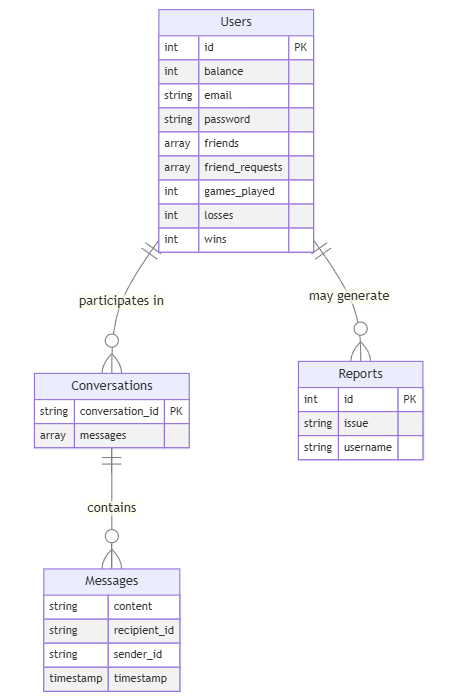
\includegraphics[scale=0.7]{finalERDdiagram.png}
    \caption{ERD Diagram of the Final Database Architecture}
    \label{fig:erd_diagram}
\end{figure}
